\chapter{Registration Pipeline using Line Features}
\label{chap:pipelinefeatures}
In this chapter we describe how the Vector-valued Gaussian Model is utilized in our implementation of a 3D Face Registration Pipeline. To enhance the registration outcome of this pipeline we use additional annotations to extend the prior correspondences given initially by the landmarks described in \ref{section:}. The additional annotations are parametric curves, we call line features, that mark key regions on the 2D colored images of a face scan. In the following we provide a description of line features and their use
as well as a description of the registration pipeline. 

\section{Line Features}
Line features serve the purpose of augmenting the quality of registration by initiating it with a set of corresponding lines. They define correspondence in feature regions of the given face scans, i.e. the eyes and ears and lips. These regions have to be accurately mapped on to one another for the registration to produce acceptable results. For this purpose we mark their contour lines with parametric curves. 
\begin{comment}so that the registration process produces an accurate mapping of the contour lines of these regions which would otherwise not be possible. Without this
information deformation fields found by the algorithm are accurate enough to produce a correct mapping and the resulting deformed templates aren't feasible substitutes for the targets. \viscomment{Und sehr spezifische zuordnung, wenn die Augenkante versetzt ist, sieht man das sofort}, because of it’s smoothness constraint.\end{comment}

We have 8 line features given for every scan we want to register. These have been marked on three images of every face, see \ref{fig:scanner}. They are made up of a set of segments, each of which is modelled with a \textbf{B\'{e}zier curve} of a specified order, see \ref{fig:linefeatures}. B\'{e}zier curves are often used in Computer
Graphics for modelling smooth curves of varying order. Given a set of control points $\mathcal{P} = \{P_{0}, P_{1}, P_{2}, \ldots, P_{n}\}$ the B\'{e}zier curve through these points is given by
\begin{equation}
    C(t)=\sum_{i=0}^{n}P_{i}B_{i,n}(t)
\end{equation}
where $B_{i,n}(t)$ is a Bernstein polynomial 
\begin{equation}
    B_{i,n}(t)=\begin{pmatrix} n \\ \\ i \end{pmatrix}(1-t)^{n-i}t^i
\end{equation}
and $t \in [0,1]$ is the curve parameter. The line features consists of multiple segments of B\'{e}zier curves. Due to the nature of the objects depicted there are open as well as closed curves, see fig. \ref{linefeatures}. 

\begin{figure}[h!]
    \centering
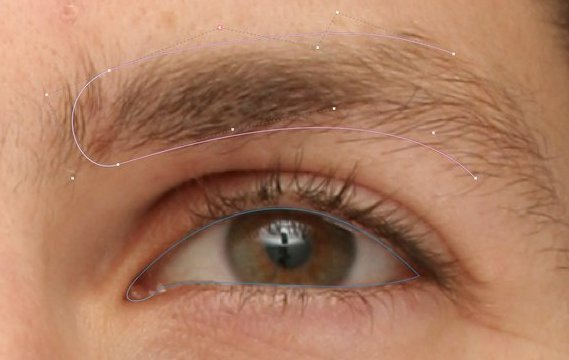
\includegraphics[width=\textwidth]{./resources/img/eyebrow_left.jpeg}
\caption{Line Features of the left eyebrow and eye, consisting of b\'{e}zier curves defined by visible control points (white). The line features are marked on 2D color images taken during scanning procedure.}
\label{fig:linefeatures}
\end{figure}

\section{Sampling 3D Points from 2D Line Features} 
The line features provide us with additional prior information about the nature of the deformation field. In order to incorporate the line features in the Vector-valued Gaussian Model, we transform them to additional point-wise information. The points are obtained by sampling the line features at discrete intervals resulting in a set of additional landmarks $L_{Add} = \{l_{1}, \cdots, l_{N}\}$. These define the mapping $\Omega:L_{Add\mathcal{M}} \rightarrow L_{Add\mathcal{T}}$ of the line features in the template face mesh on to those in the target face mesh.\\
Establishing correspondence for a pair of ears for example is very difficult, even for
experts, because of their very different topology. The structure of the concha is very
complex. For this reason, we define correspondence between lips, eyes and ears through the contour lines of their rims. Further modelling the ratio between the different parts of these contours would again be tedious. Therefore, we simplify the assumptions for similarity to an equidistant parametrization of the line features so that the mapping $\Omega$ is approximately plausible. In effect, when a curve is sampled at $n$ points, these $n$ points are all at equal parametric intervals.
\begin{comment}
Bei den Ohren ist die Korrespondenz wirklich schwierig und auch als Mensch je nach Ohrenpaar kaum zu bestimmen. Gerade die Struktur der Ohrmuschel kann wohl nicht immer in korrespondenz gebracht werden. Jedoch sind alle Ohren durch eine äussere Linie begrenzt und die wollen wir matchen. Nun ist es in der Tat so, dass nicht immer alle Ohrläppchen gleich gross sind oder markante Krümungen der äusseren Ohrlinie an der gleichen Stelle auftreten. Wir ignorieren dies jedoch / bzw wir
vereinfachen dies durch unsere Äquidistantz Annahme und sagen dies sei dann genügend gut registriert und störe das Model das wir bauen nicht zu sehr.
\end{comment}
\def\earpathf{(-1,1.5) .. controls (-1,2.3) and (1,2.8) .. (1,1.5) .. controls (1, -.2) and (0.3,-.1) .. (0.3,-1) .. controls (0.2,-1.5) and (-.5, -1.7) .. (-1,-1.25);}
\def\earpathl{(3,2) .. controls (3,3.3) and (5.6,3.7) .. (5.6,2) .. controls (5.6, 0) and (4.6,0) .. (4.6,-1.3) .. controls (4.6,-2) and (3.5, -2) .. (3,-1.5);}

\begin{figure}[h!]
    \centering
    \begin{tikzpicture}
        \draw[black]\earpathf
        \fill (-1,1.5) circle[radius=2pt];
        \fill (0.1,2.3) circle[radius=2pt];
        \fill (1,1.5) circle[radius=2pt];
        \fill (0.8, 0.25) circle[radius=2pt]; 
        \fill (0.3,-1) circle[radius=2pt];
        \fill (-1,-1.25) circle[radius=2pt];
        \draw[black]\earpathl
        \fill (3,2) circle[radius=2pt];
        \fill (4.3, 3.12) circle[radius=2pt];
        \fill (5.6,2) circle[radius=2pt];
        \fill (5.25,0.35) circle[radius=2pt];
        \fill (4.6,-1.3) circle[radius=2pt];
        \fill (3,-1.5) circle[radius=2pt];
        \draw[ultra thick, blue, ->] (-.8,1.5) -- (2.8,2);
        \draw[ultra thick, blue, ->] (1, 0.25) -- (5.1, 0.35);
        \draw (1.8, .9) node {\Large\textcolor{blue}{$\Omega$}};
        \draw (-1,.5) node {line feature of $\mathcal{M}$};
        \draw (4,1.2) node {line feature of $\mathcal{T}$};
    \end{tikzpicture}
    \label{fig:DiffEars}
    \caption{Mapping of equidistant samples of \textbf{ear} line features from the reference (left) on to the target (right)}
\end{figure}

\subsection{Arc Length Parametrization}
The underlying parameter $t \in \mathbb{R}$ of a b\'{e}zier curve segment of a single line features is dictated by the curve's velocity. In order for us to be able to sample the line feature in equidistant intervals, however, the parameter has to be linear in respect a the curve segment's length. In consequence, we have to compute an equidistant parametrization for each of the curve segments of a line feature before sampling it.
\def\earpathf{(-1,1.5) .. controls (-1,2.3) and (1,2.8) .. (1,1.5) .. controls (1, -.2) and (0.3,-.1) .. (0.3,-1) .. controls (0.2,-1.5) and (-.5, -1.7) .. (-1,-1.25);}
\def\earpaths{(3,1.5) .. controls (3,2.3) and (5,2.8) .. (5,1.5) .. controls (5, -.2) and (4.3,-.1) .. (4.3,-1) .. controls (4.2,-1.5) and (3.5, -1.7) .. (3,-1.25);}
\begin{figure}[h!]
    \centering
    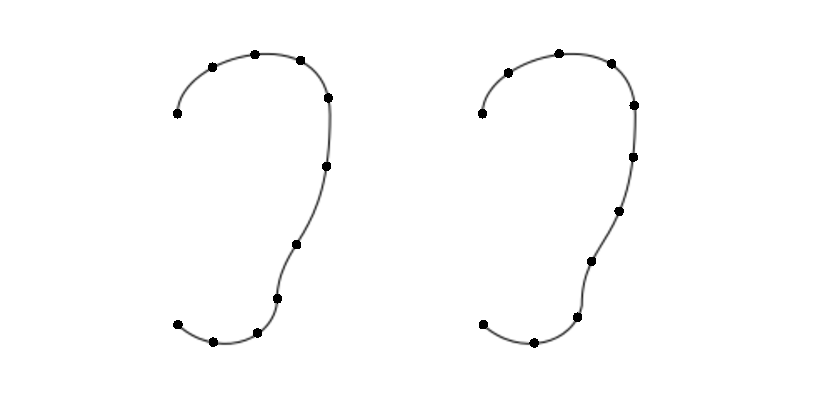
\includegraphics{./resources/figures/ears_diffparam.pdf}
    \label{fig:diffparam}
    \caption{a simplified - the depicted \textbf{ear} line feature is treated as one sole b\'{e}zier segment - illustration of the difference between b\'{e}zier (\textbf{left}) and equidistant (\textbf{right}) parametrization.}
    \begin{comment}
    \begin{tikzpicture}
        \draw[black]\earpathf
        \draw[black]\earpaths
        \fill (-1,1.5) circle[radius=2pt];
        \fill (0.1,2.3) circle[radius=2pt];
        \fill (1,1.5) circle[radius=2pt];
        \fill (0.8, 0.25) circle[radius=2pt]; 
        \fill (0.3,-1) circle[radius=2pt];
        \fill (-1,-1.25) circle[radius=2pt];

        \fill (3,1.5) circle[radius=2pt];   
        \fill (3.3,2) circle[radius=2pt];
        \fill (4.1, 2.3) circle[radius=2pt];
        \fill (4.85, 2) circle[radius=2pt];
        \fill (4.99, 1.4) circle[radius=2pt];
        \fill (4.85, 0.4) circle[radius=2pt];
        \fill (4.4, -.45) circle[radius=2pt]; 
        \fill (4.3, -1.05) circle[radius=2pt]; 
        \fill (3.9, -1.45) circle[radius=2pt]; 
        \fill (3,-1.25) circle[radius=2pt];
    \end{tikzpicture}
    \end{comment}
\end{figure}
The solution to this problem is based on the respective curve's arc-length, which is defined as the length of the rectified curve. The underlying parameter $t$ must then correspond - at every point of the curve - to the ratio between the length of a fraction of the curve $l$ and the total curve length $L$: $t = \frac{l}{L}$.

\paragraph{In theory}
It is possible to get the arc length $L(t)=\int_{t_{0}}^{t_{1}} \left|C'(t)\right| dt$ for given parameters $t_{0}, t_{1}$ where $C'(t)$ is the derivative of the curve $C:t \in [0,1] \rightarrow \mathbb{R}^2$. We, however, want to find a reverse mapping from the length of a fraction of the curve $l$ to the curve parameter $t = L^{-1}(l)$. 
Instead of deriving this function analytically we decided to use a numeric approximation.
\paragraph{In practice}
As we are not in need of a subpixel resolution, we can skip the formal math and use a lookup table to compute the arc-length. First, we calculate a large number of points on each segment of the curve using the parametrization of the corresponding B\'{e}zier curve. For each sampled point, we save a key-value-pair to a new entry of the lookup table. The approximate distance of the point from the origin of the segment is inserted as the key, while the point's coordinates are stored
as the value. 
\begin{figure}[h!]
\centering
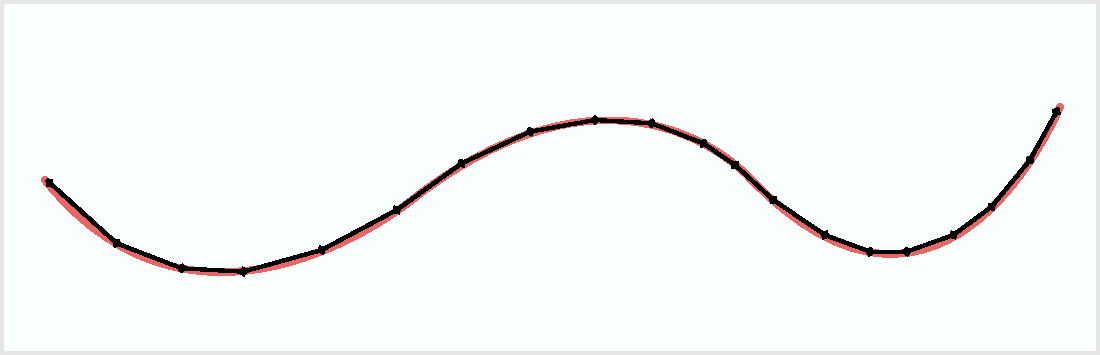
\includegraphics[width=\textwidth]{./resources/figures/distance_computation.pdf}
\label{fig:lookup}
\caption{Visualization of euclidean distances between points computed with a b\'{e}zier curve parametrization. This is an arbitrary line feature used solely for demonstration purposes.}
\end{figure}
The distance is approximated by summing up the euclidean distances of each point to its respective predecessor starting from the origin. The resulting lookup table contains the approximate distances and coordinates of a large number of points from the origin of a curve segment. Assembling the segments' lookup results in the lookup table of the whole curve, where the last key represents the curve's arc-length. Through this procedure we have gained an indirect mapping from the length of a fraction of the curve to the parameters of the B\'{e}zier curve segments via the point coordinates.\\ 
In a second step, the curve can easily be sampled by computing the length of parametric intervals $\frac{L}{N}$ for a specified number of points N.\\
$l=k \cdot \frac{L}{N}$ returns the current length of the curve for the sampling point of index k, where $k=[0,\cdots,N]$ for open curves and $k=[0,\cdots,N-1]$ for closed curves.
To get the point coordinates for a fraction of the curve, we now simply perform a binary search on the lookup table for its approximated distance from the origin $l$. We choose the index which returns the coordinates for the exact fraction length and if this requirement can't be met the index with the next smaller length. The returned point coordinates are used as the approximate coordinates of the sought sample point.
\subsection{3D Mesh Projection of Sampled Points}
Having implemented arc length parametrization it is possible to draw an arbitrary amount of sample points $p \in \mathbb{R}^2$ from the 2D line features. These are defined as a set of points $S \subset \mathbb{R}^2$. Our goal is to use these additional points as landmarks describing the features on the 3D mesh of the corresponding face. To achieve this we have to project the sampled points of each line feature on to the corresponding face mesh in order to obtain
their approximate 3D representation. We use this method because we have no information on the depth of the respective line feature.  
In the camera model - derived from the callibration of the scanner - the image is located on the viewing plane or viewport along the z-axis from the focal point. The idea is to follow the direction of a point on the line feature - which lies in the viewport - from the focal point and obtain a projection on to the face mesh along this direction. We want to use the discrete mesh of a given face scan to create a new vertex that is the most accurate representation of the sample point on
the line feature. In order to find vertices with similar directions to the sample direction, we save all the distances of mesh vertices in a list for which a similarity measure is higher than a specified threshold. As the similarity measure we use the dot product of normalized vertex and sample directions. We then select the distance of the vertex with the highest similarity. Finally, we project the distance of this vertex onto the direction of our sample point and thereby obtain an approximation of the points position in the mesh. A new vertex is created at this location. %\begin{wrapfigure}[]{o}[2cm]{\documentwidth}
\begin{figure}[h!]
    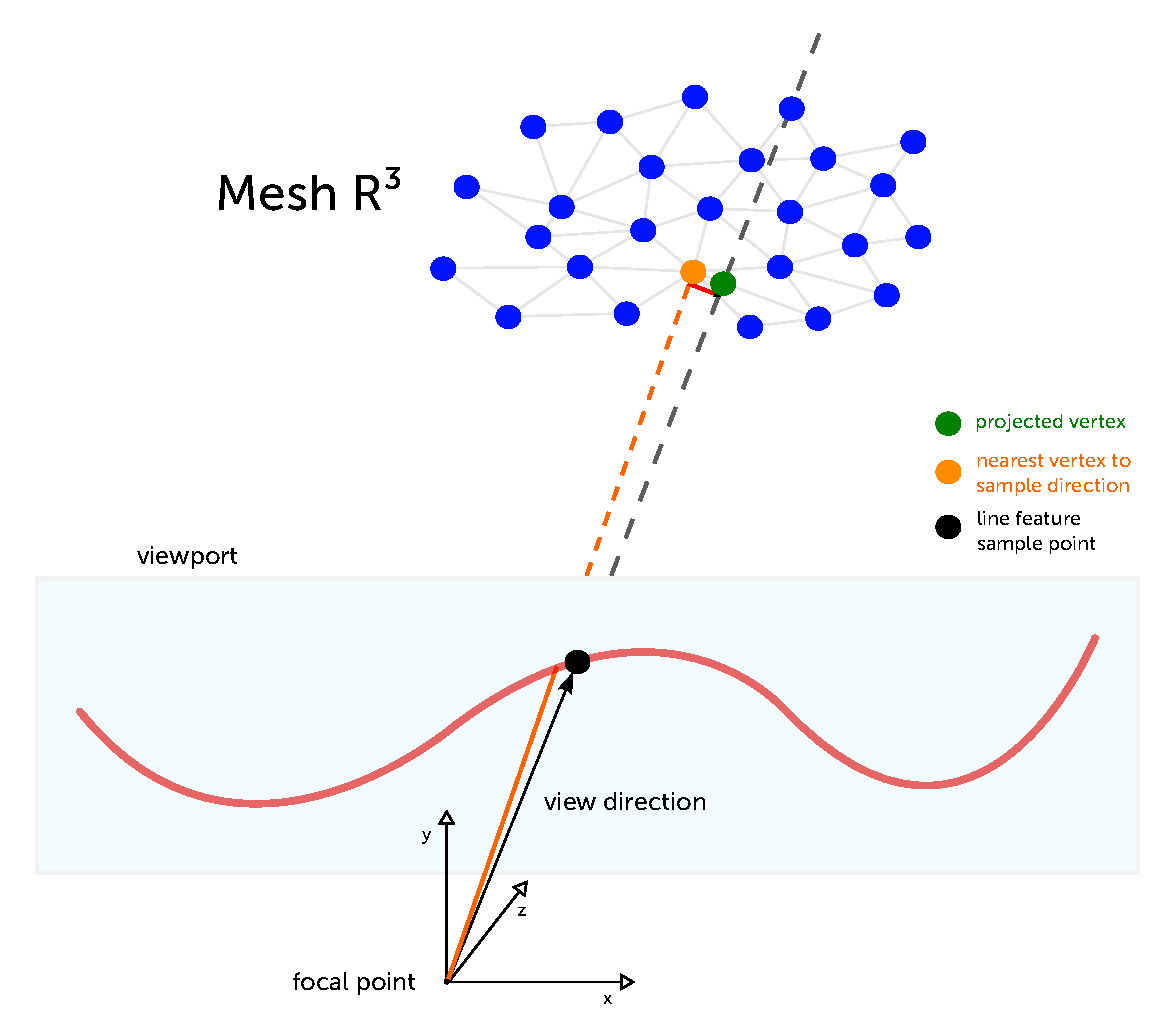
\includegraphics[width=\textwidth]{./resources/figures/projection.pdf}
\label{fig:projection}
\caption{shows the projection of a sample point - on a 2D line feature - from the viewport onto a triangulated 3D mesh. The distance vector of the vertex with the most similar direction vector (orange) is projected (red) onto the direction of the sample point (black arrow), resulting in the projected vertex (green)}
\end{figure}
\subsection{Preparing the Template Mesh}
For the line features projected on to the scans to be of use, line features also have to be marked on the template mesh. We use the mean mesh of a 3D Morphable Model [http://gravis.cs.unibas.ch/publications/2009/BFModel09.pdf] as the template mesh.

We render three different images, similar to those taken during the scanning of the faces, for marking the line features.
The 2D line features can then be projected back onto the mesh using the rendering parameters. With the projection we obtain the corresponding, equidistant samples of the line features on the template. They obtained additional prior information is used in the registration algorithm to define the posterior deformation model and to produce better registration results.
\begin{figure}[h!]
    \centering
    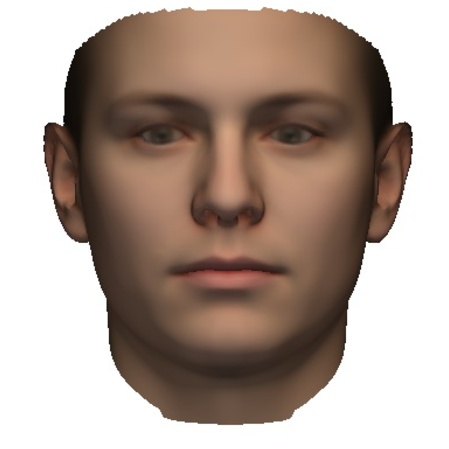
\includegraphics[width=.3\textwidth]{./resources/img/mean_msh.pdf}
    \caption{Mean mesh of the Basel Face Model}
\end{figure}

\begin{figure}[h!]
\centering
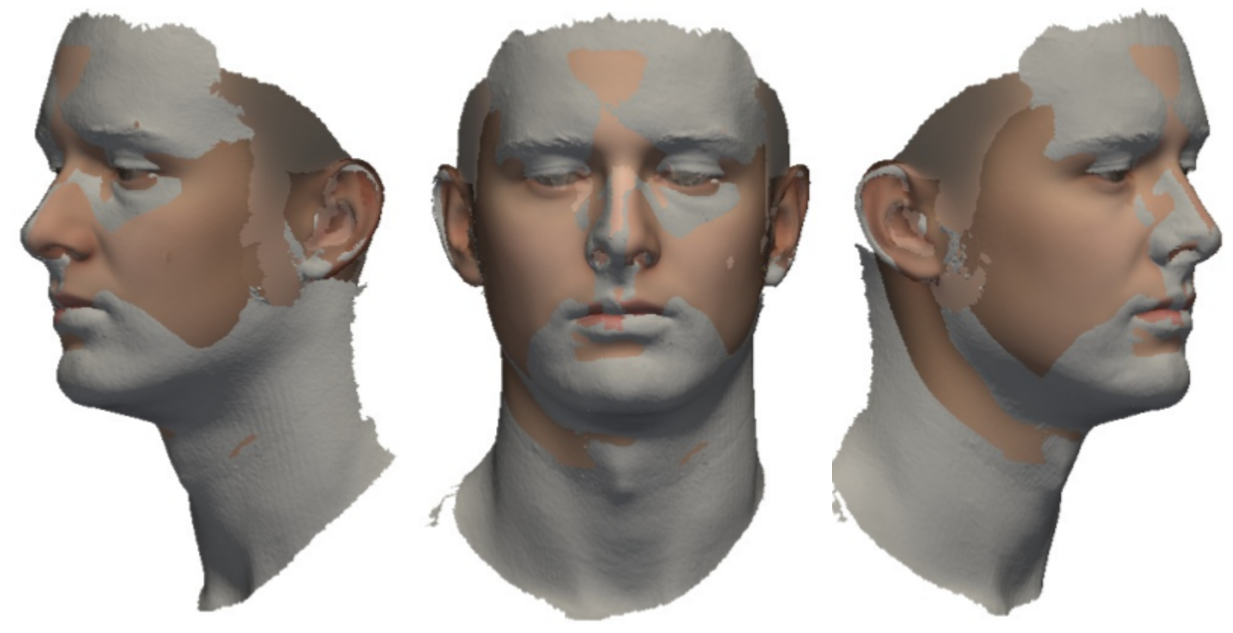
\includegraphics[width=.8\textwidth]{./resources/img/overlap_mean_target.pdf}\\
\caption{Overlap of textured mean template with a target scan (gray surface)}
\label{fig:overlap}
\end{figure}

\section{Rigid Mesh Alignment}
Before we can start creating Gaussian Models, we first have to ensure that each target is aligned with the template. After all, we want to model the variability of different faces without incorporating an additional offset. We therefore have to perform a rigid transformation constisting of a translation and a rotation to align the template and target meshs according to their landmarks. To compute the transformation we use the set
of landmarks pairs whose identifiers exist for both meshs. The targets are clipped at the neck and around the ears where the scanner has produced artifacts. The computed transformation is then applied to all vertices of the respective face scan to align it with the template. The aligned mesh pair serves as the starting point for the actual registration, see fig. \ref{fig:overlap}.\newline
\newline

\begin{figure}[h!]
\centering
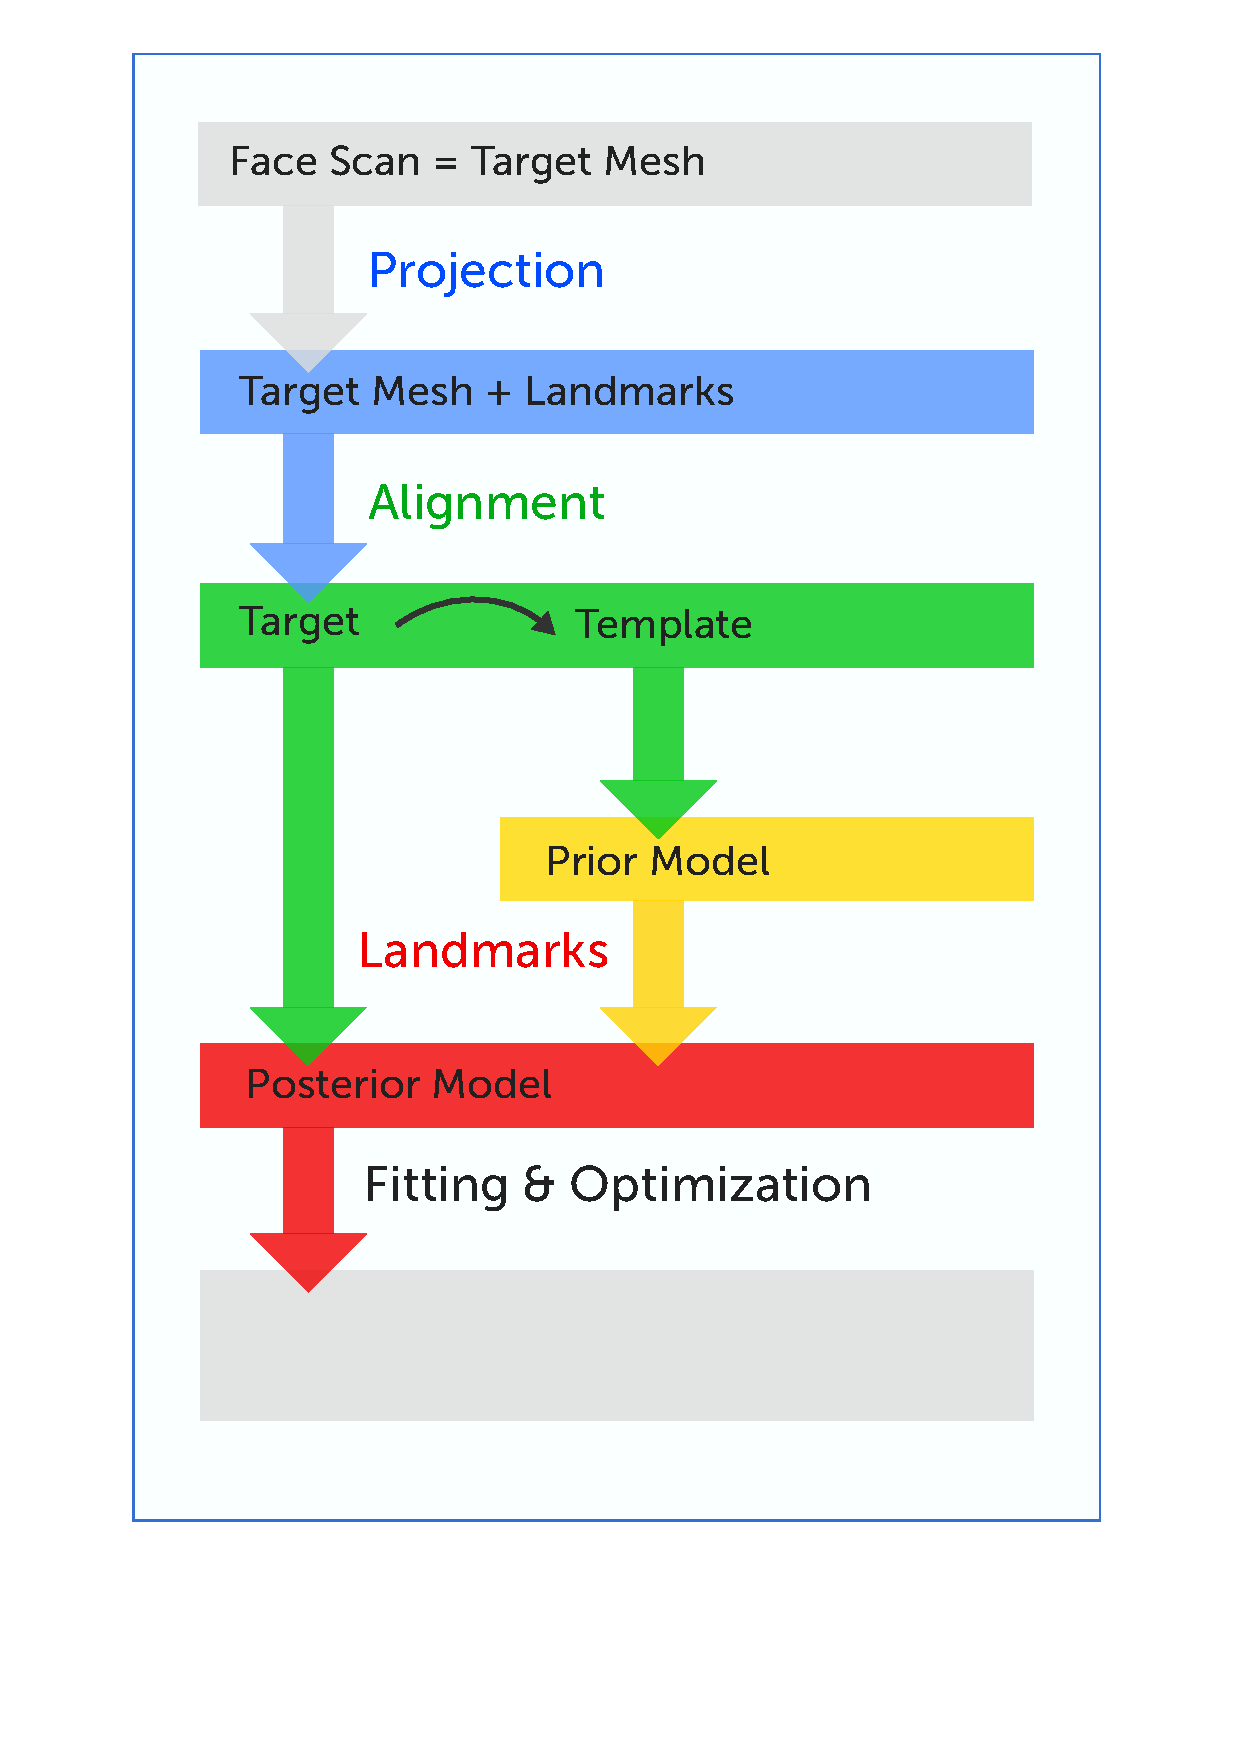
\includegraphics[width=.9\textwidth]{./resources/figures/pipeline.pdf}
\label{fig:pipeline}
\vspace{-20pt}
\caption{An overview of the different stages of the registration pipeline with an examplary visualization of face meshs at every stage.}
\end{figure}

We are now set for the actual registration involving the computation of the Prior and Posterior Gaussian Models and the Fitting of the Posterior Model to a face scan. For the definition of the Gaussian Process distributions we use statismo \ref{bib:statismo}. It is a framework for PCA based statistical models. These are used to describe the variability of an object within a population, learned from a set of training samples. We use it to generate a statistical
model of the template mesh equaling the parametric representation of the Gaussian Process Posterior described in sec. \ref{sec:optimization}. 

\begin{figure}[h]
\centering
\subfloat[sample of the GP Prior]{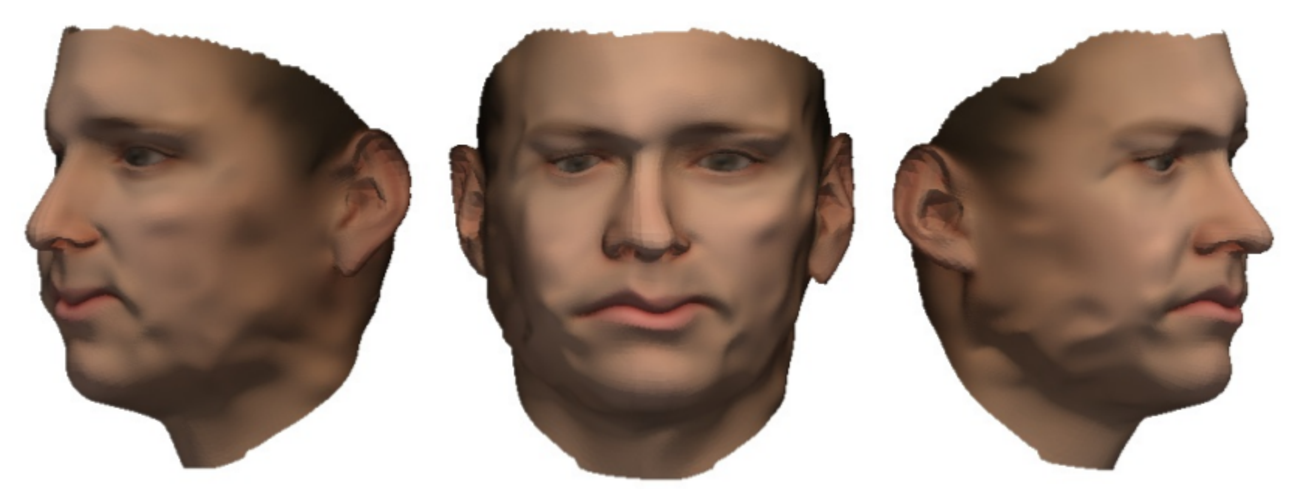
\includegraphics[width=.8\textwidth]{./resources/img/prior_sample_2_profile.pdf}}\\
\subfloat[sample of the GP Prior]{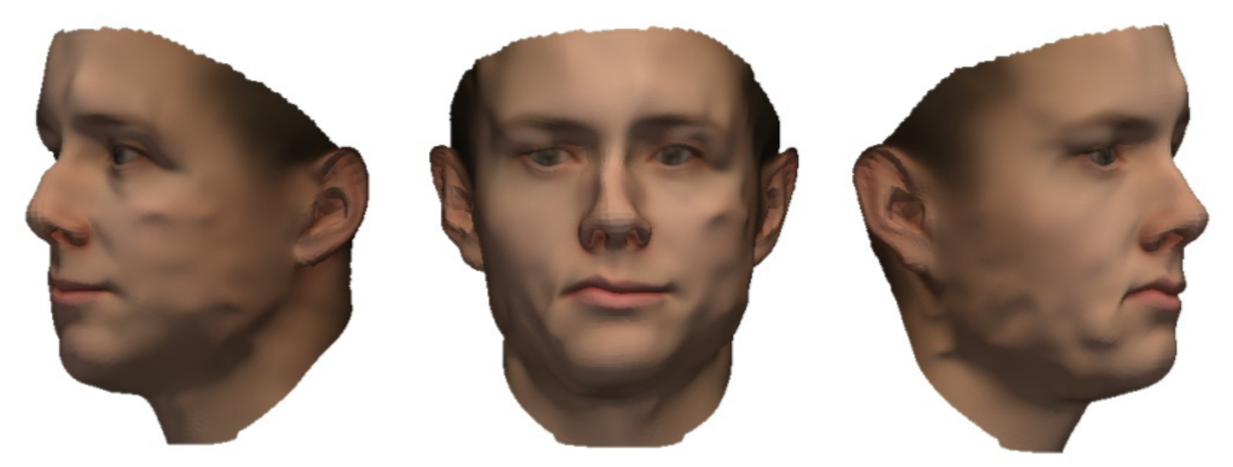
\includegraphics[width=.8\textwidth]{./resources/img/prior_sample_3_profile.pdf}}
\label{fig:priorprofile}
\caption{Prior faces computed from samples drawn from the Gaussian Process Prior Model. The deformations are not truely face-like, because they are only modeled through the covariance of the template mesh vertices.}
\end{figure}

\section{Prior Model}
After aligning the target with the template mesh, we define a distribution of possible deformations of the template mesh, as described in \ref{chap:GP}. This Gaussian Process (GP) Prior distribution is represented as a statistical model. This allows for samples to be drawn from this representation. These samples are 3D face meshs that are the result of the deformations generated by the GP Prior and added to the template mesh for visualizations, some of these prior faces are displayed in fig. \ref{fig:priorprofile}. The deformations are up until now defined solely on the ground of the covariance of the template mesh points.

\section{Posterior Model}
The deformations generated by the GP Prior are of course not admissible. We receive admissible deformations by adding the target landmarks and the additional set of sampled line features to the GP Prior distribution. Using statismo we create a statistical model, which is partially fixed at the target landmarks, from the template mesh. Now we have incorporated the given prior information, we obtain a model that leads to meshs that are more face-like.

\begin{figure}[h]
\centering
\subfloat[sample of GP Posterior]{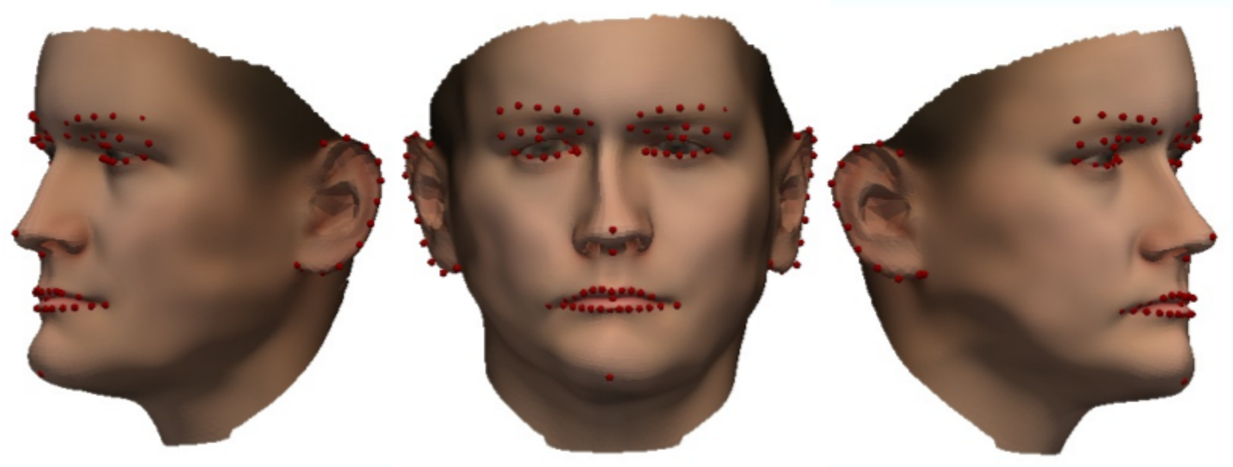
\includegraphics[width=.8\textwidth]{./resources/img/posterior_sample_17.pdf}}\\
\subfloat[sample of GP Posterior]{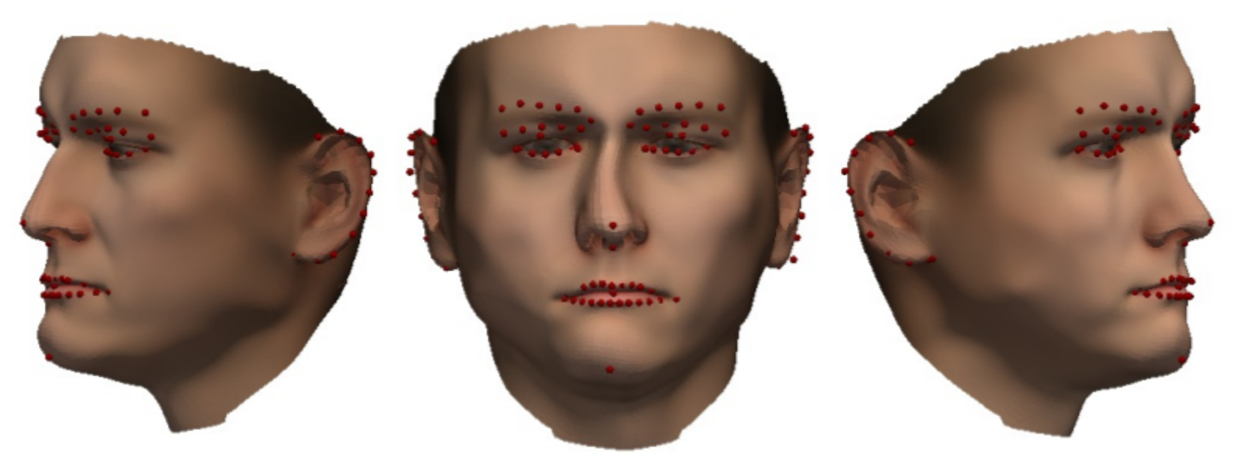
\includegraphics[width=.8\textwidth]{./resources/img/posterior_sample_23.pdf}}
\label{fig:posteriorsample}
\caption{Posterior faces computed from samples drawn from the GP Posterior. The resulting faces are considerably more face-like than those in fig. \ref{fig:priorprofile}}
\end{figure}

\section{Optimization of the Posterior}
In order to optimize the respective GP Posterior Models of the template according to the target scans, we obtain the parametric representation of the GP Posterior Model using statismo. We then use the limited-memory BFGS optimization build into the Insight Toolkit (ITK). Optimize parameters for the set of chosen basics functions in the parametric model. First we used the Mena Squared Error as the loss function. However, this estimator did not yield desirable results, as can be seen in \ref{fig:msquaresfit}.
\begin{comment}
\viscomment{Überarbeiten}
Before starting the optimization we again use the statismo framework to obtain the parametric representation of the GP Posterior Model of the template. This part of statismo framework built on the Insight Toolkit (ITK) is used to optimize the parameters for the set of chosen basis functions. In each step the optimizer computes the parameters that cause a minimum in a specified similarity measure. We used the mean squared error (MSE) as a similarity measure. This process is reiterated until the similarity measure stays within a tolerance interval for a fixed
number of iterations.
\viscomment{Schema of ITK optimizer?}
\end{comment}
\begin{figure}[h!]
\centering
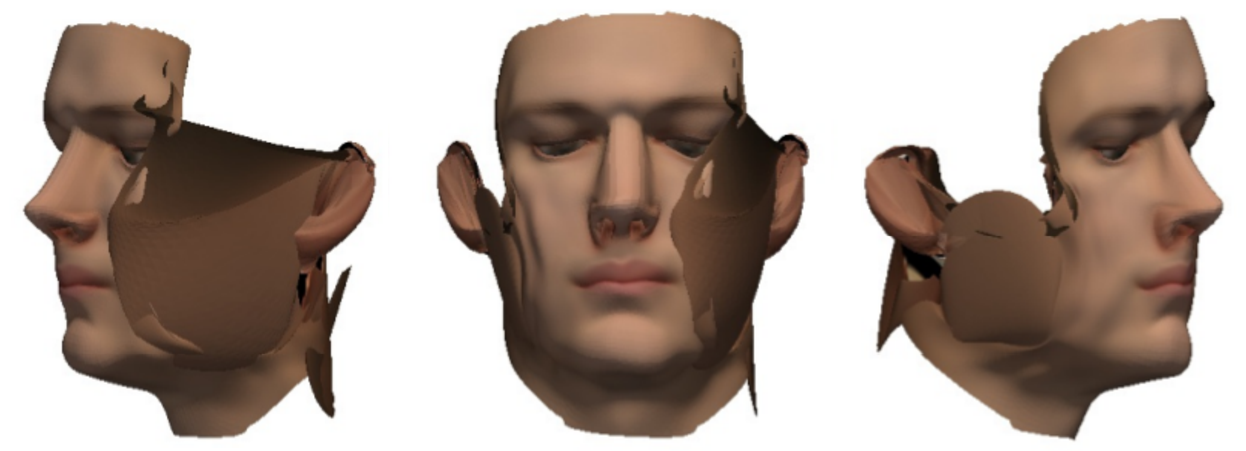
\includegraphics[width=.8\textwidth]{./resources/img/00029_meansquares_fit.pdf}
\label{fig:msquaresfit}
\caption{A fit of the template mesh obtained using the Mean Squared Error as the distance metric. The deformation in the regions where template and target do not overlap cause major distortions in the resulting fit.}
\end{figure}
The reason for the bad performance of MSE is that after the alignment of template and target mesh, the template protrudes over the target on both sides of the head, consult in fig. \ref{overlap}. Performing optimization as described in \ref{sec:optimization} using the simple MSE as a distance measure between the template and target mesh penalizes the portruding regions of the template with a strong gradient towards the rims of the template and therefore causes strong distortions. 

\section{Robust Loss Functions}
To overcome the problems described above, we tried a range of different robust estimators, namely the Tukey, Huber, and Fair estimators. The advantage of these
estimators lies therein that they are less sensitive to outliers, reducing registration artifacts considerably. Outliers are in this case template mesh points that are farther away than a certain threshold from the next point on the target mesh. However, these techniques require parameter tuning to first which produce reasonable/acceptable visual results.

Fair
\begin{subequations}
\begin{equation}
\rho(x)=c^2\left[\frac{\left|x\right|}{c}-log(1+\frac{\left|x\right|}{c})\right]
\end{equation}
\begin{equation}
    \psi(x)=\frac{x}{1+\frac{\left|x\right|}{c}}}
\end{equation}
\end{subequations}
Huber
\begin{subequations}
\begin{equation}
    \rho(x) = \twopartdef {\frac{x^2}{2}} {\left|x\right|<k} {k(\left|x\right|-\frac{k}{2})} {\left|x\right|\geq k}
\end{equation}
\begin{equation}
    \psi(x) = \twopartdef {x} {} {k sgn(x)}{} 
\end{equation}
\end{subequations}
Tukey
\begin{subequations}
\begin{equation}
    \rho(x) = \twopartdef {\frac{c^2}{6}\left(1-\left[1-\left(\frac{x}{c}\right)^2\right]^3\right)} {\left|x\right|\leq c} {\frac{c^2}{6}} {\left|x\right| > c}
\end{equation}
\begin{equation}
    \psi(x) = \twopartdef {x\left[1-\left(\frac{x}{c}\right)^2\right]^2} {} {0} {}
\end{equation}
\end{subequations}

\begin{figure}[h!]
\centering
\subfloat[target with mean texture applied]{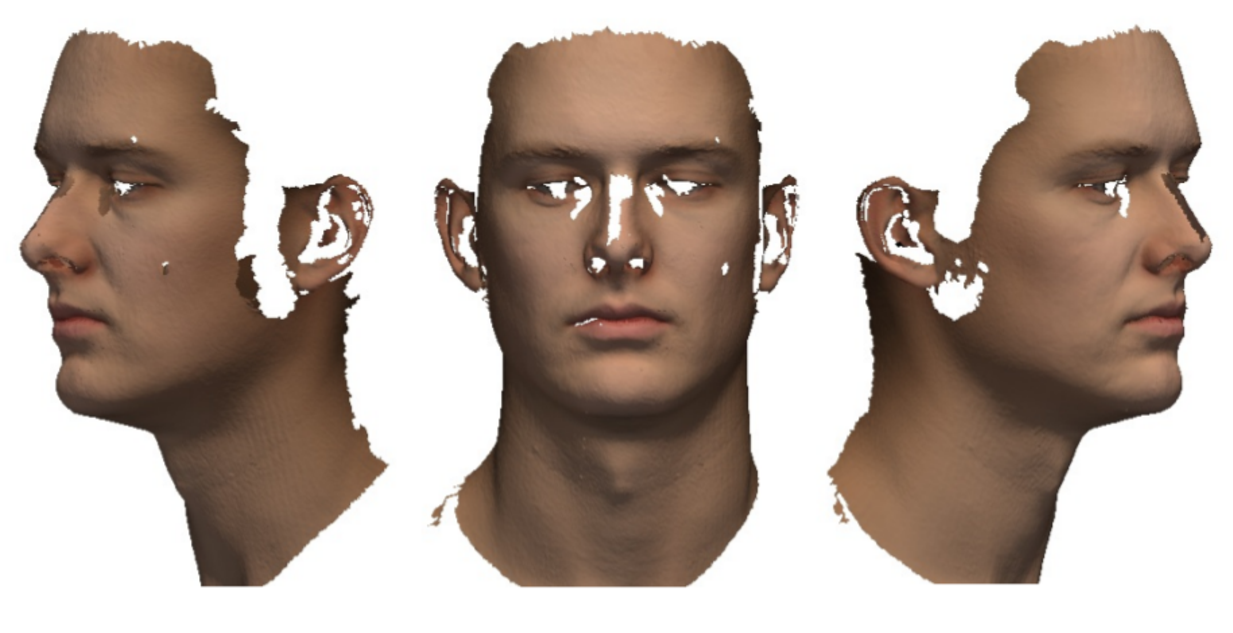
\includegraphics[width=.8\textwidth]{./resources/img/00029_textured_target.pdf}}\\
\subfloat[optimized mean posterior fit]{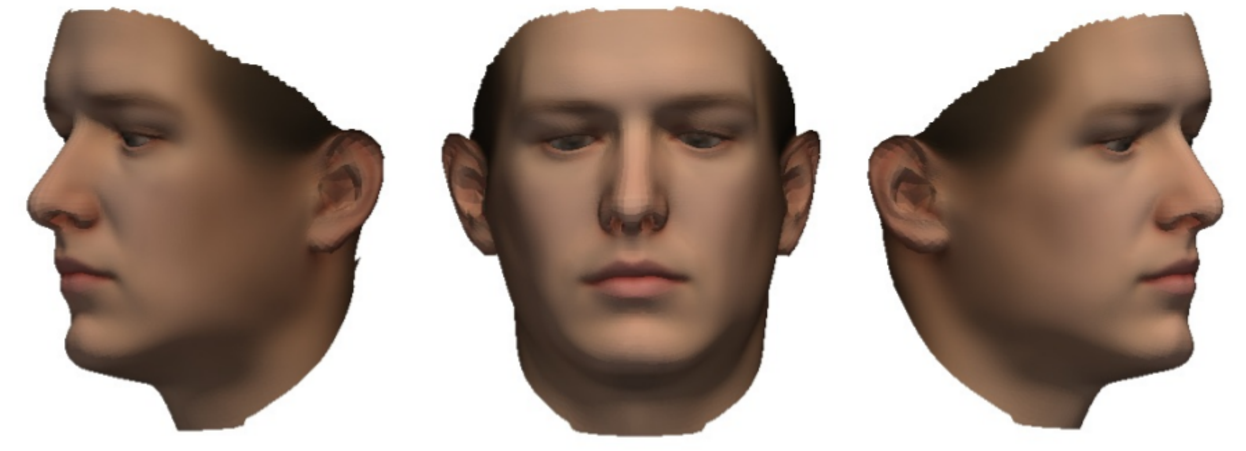
\includegraphics[width=.8\textwidth]{./resources/img/00029_fit.pdf}}
\label{fig:fitcomparison}
\caption{The fitting result in a) was obtained with the Tukey estimator, parameter c=7.0. The texture of the mean mesh has been applied to the target to make the meshs comparable. The fit in a) has considerable likeness to the target b), although it lacks expressiveness}
\end{figure}

\begin{comment}
\section{A more complex Noise Model}
additive i.i.d Gaussian Noise ---> Different variance for every landmark and line feature id
\end{comment}
